\documentclass[twoside, 11pt, a4paper]{article}

%%%%%%%%%%%%%%%%%%%%%%%%%%%%%%%%%%%%%%%%%%%%%%%%%%%%%%%%%%%%%%%%%%
% Any additional packages needed should be included after csmr.  %
% Note that csmr.sty includes epsfig, amssymb and graphicx,      %
% and defines many common macros, such as 'proof' and 'example'. %
%%%%%%%%%%%%%%%%%%%%%%%%%%%%%%%%%%%%%%%%%%%%%%%%%%%%%%%%%%%%%%%%%%

\usepackage{csmr}
\usepackage[cp1250]{inputenc}
\usepackage{fancyhdr}

% Definitions of handy macros can go here

%\newcommand{\dataset}{{\cal D}}
%\newcommand{\fracpartial}[2]{\frac{\partial #1}{\partial  #2}}

% Heading arguments are {volume}{nmber}{submitted}{published}{author-full-names}

\csmrheading{1}{1}{2010}

% Short headings should be running head and authors last names

\ShortHeadings{1}{1}{2010}{Instructions for Formatting CSMR article.}{Sorici, B\u{a}l\u{a}nel}

\begin{document}

\title{The use of Adaptive Culture Models in Collective Behavior}

\author{\name Alexandru Sorici, Anca B\u{a}l\u{a}nel\\
       \addr University POLITEHNICA of Bucharest\\
       Faculty of Automatic Control and Computers, Computer Science Department\\
       \email Emails: alex.sorici@gmail.com, anca.balanel@gmail.com}

\maketitle

\begin{abstract}
Social behavior as an emergent phenomenon, rather than as a reflection of social structure and enforcements, is gaining attention not only from sociologists, but also from the computer science area. Simulations are performed in order to understand how cultures form, why they are different and how they evolve over time. This paper presents an existing agent based model of culture dissemination in the context of collective behavior. We implement some of its extensions with the purpose to find potentially interesting properties that emerge from a given set of rules that govern the specific settings. Social behavior as an emergent phenomenon, rather than as a reflection of social structure and enforcements, is gaining attention not only from sociologists, but also from the computer science area. Simulations are performed in order to understand how cultures form, why they are different and how they evolve over time. 
\end{abstract}

\begin{keywords}
self-organization, emergence, culture models, collective behavior
\end{keywords}

\section{Introduction}

In anthropology there are many ideas about the nature of \emph{culture}. Cultural models, according to Roy D'Andrade, are used to \emph{represent something}, or to \emph{reason with} by mentally manipulating the parts of the model to solve some problem. They are learned knowledge, and their learning is social and individual. \emph{Culture} is thought to be composed of many cultural models, differentially internalized by culture members. Modelling collective behavior and cultures can find one possible application in the field of intercultural relations management, within a society or corporation.

Computational models of human collective behavior offer promise in providing quantitative and empirically verifiable accounts of how individual decisions lead to the emergence of group-level organizations. \emph{Agent based models} (ABMs) describe interactions among individual agents and their environment, and provide a process-oriented alternative to descriptive mathematical models. 
This work analyzes and presents the outcomes of several experiments based on a model of culture dissemination (as introduced by Robert Axelrod).
The following section gives a view on the main existing approaches towards an agent based society model and provides some examples. It also describes Axelrod's model which serves as a basis for our experiments. Section 3 explains the main goals and settings of the experiments.


\subsection{State of the Art}

ABMs build social structures in a 'bottom-up' fashion, by simulating individuals by virtual agents, and creating emergent organizations out of the operation of rules that govern interactions among agents. 

Agent-based models possess important characteristics such as: computational description at the level of agents, stigmergetic interactions (communication through the environment), autonomous behavior of agents and the possibility of spatially distributing agents. These allow for a more flexible and intelligible way of analyzing emergent behavior (as opposed to a descriptive mathematical models approach).

In the model proposed by Axelrod \cite{Axelrod97}, the similarity between individuals influences their interactions, and interactions result in individuals adopting traits from one another. The agent-based model reveals the global effects of social influence: dissemination of culture, while preserving a few key differences.
Axelrod has theorized that similarity between pairs of individuals can result in the spread of culture. In his simulations, individuals are represented as strings of symbols called "features"; the number and length of the strings and the universe of symbols available to them are parameters of the system. Axelrod postulates that the probability of human interaction is a function of the similarity of two individuals: \textit{"The basic idea is that agents who are similar to each other are likely to interact and then become even more similar"} (Axelrod, 1997).

The dynamics of the model are the following:
\begin{itemize}
\item An active agent an one of its neighbors are randomly chosen
\item The agents interact with probability equal to their cultural similarity: the active agent copies the value of a feature on which it and its neighbor's value differ (if there is such a feature).
\end{itemize}
The process repeats for a given number of iterations.

In Axelrod's model, culture is viewed as subject to social influence. Latan\'e's social impact theory \cite{Latane} states that the behavior of an individual is influenced by the characteristics of the group he adheres to. The behavior is determined as a function of the \textbf{Strength}, \textbf{Immediacy}, and \textbf{Number} of people participating in the influencing group. Latan\'e's simulations and studies show that dynamic social impact possesses 4 predominant characteristics:

\begin{itemize}
\item \textit{Consolidation}: The diversity of opinions is reduced as individuals are exposed to a preponderance of majority arguments
\item \textit{Clustering}: People become more similar to their neighbors in social space (usually correlated with physical space in Latan\'e's view).
\item \textit{Correlation}: Attitudes that were originally independent tend to become associated.
\item \textit{Continuing diversity}: Clustering protects minority views from complete consolidation.
\end{itemize}

All in all, the theory explains that as people interact they persuade one another of things, they show one another how to do things, they impress one another, they copy one another, and the simple, obvious result is they become more similar.

The concept of similarity that begets similarity is also central to Axelrod's \textit{Dissemination of Culture} study \cite{Axelrod}. The paper sets similarity as a causality for social interaction and influence. It is interesting to note that the work also shows how variations of the model's central parameters (number of features, number of traits per feature, range of interaction, size of territories) impact the emergence of regions of shared culture or the achievement of cultural uniformity.

A \emph{cultural region} can be defined as a set of contiguous sites (cells) with an identical culture. Simulations presented in \cite{Axelrod} show the emergence of regions of shared culture, over time. 
A \emph{stable region} is a cultural region that exists even if it has nothing in common to the adjacent regions. It is interesting to see, for a society, how many stable regions will survive over a given period of time. Experiments have proved that the number of stable regions that survive is influenced by variation of the model parameters.

Based on the four central model parameters, two of the results proved to be intuitive, whereas the other two were more surprising. Intuitively, the number of stable regions increases with the number of possible traits per feature (greater diversity), and decreases with the range of interaction (greater uniformity). The counter-intuitive results were that the number of stable regions decreases with more cultural features and with large territories.

Axelrod mentions many possible extensions to his original model. Examples include: cultural drift (modeled as spontaneous change in a trait), cultural attractiveness (some traits are less likely to change than others), technological change (introduction of new features or more attractive traits) or cultural divergence (interaction between dissimilar sites causes greater cultural distance).

\section{Proposed Approach and Experiments}

Our testing and experimentation framework is based on the above mentioned model of culture dissemination developed by Axelrod. Particularly, we have three main objectives.

\paragraph*{}The first objective was to establish a baseline experimental setup whose result was the duplication of the outcomes described in \cite{Axelrod}. This means that we created a population of agents wherein each individual has a set of features. Each feature has an associated integer set (its traits) from which it can take values. The interacting individuals are chosen randomly. If \textit{Ag1} interacts with \textit{Ag2}, \textit{Ag1} copies the value of a non-matching feature from Ag2 (hence they become more similar). The interacting agents must be in neighboring cells.
\paragraph*{}A modification that we brought to this first experiment was to make the interaction between individuals occur in proportion to the similarity of their features. Thus, if \textit{S} is the number of matching feature values between agents \textit{Ag1} and \textit{Ag2} and N is the total number of features then \textit{Ag1} and \textit{Ag2} have a probability of \textit{S/N} to interact. If they do interact, \textit{Ag1} will copy the value of a non-matching feature from Ag2 (hence they will become more similar). 

\paragraph*{}The second objective was to duplicate a more complicated setup which relies on a modification of Axelrod's model as described in \cite{Kennedy01}. This setup changes the way in which agents influence each other and copy traits from one another. Instead of relying on the similarity between their features, agents must strive to obtain an equilibrium between two subsets of their features. An agents features are again modeled as an array of integer values. Let us assume that an agent has 5 features and that it must strive to achieve equality between the sum of the first three features and the last two. Thus, an agent with the string 34153 would satisfy the requirements \textit{(3 + 4 + 1 = 5 + 3)}. Now, given two agents \textit{Ag1} and \textit{Ag2}, \textit{Ag1} will copy the trait from a non-matching feature, if the difference of its two subsets is greater than that of Ag2 (Ag1 has a more consistent set of features). As shown in \cite{Kennedy01}, the interpretation of this simulation is that a string may be seen as a set of features, attitudes, or beliefs held by an individual, which must be internally consistent in order to become stable. The features are also constrained to be externally consistent, that is, individuals strive to resemble their neighbors, at least when the neighbors are relatively successful at attaining a "good" set of features.

\paragraph*{}The second objective was the premise for the third one, which sees the implementation of an experiment based on the extensions proposed by Axelrod to his original model. We added the notions of \emph{cultural attractiveness} (some traits are less likely to change than others) and \emph{technological change} (introduction of new features or more attractive traits) to the modification described in the previous objective. Thus, the model that we analyzed is a combination of two proposed modifications to the original hypotheses. 
\emph{Technological change} is expressed by adding two features to the individuals in a chosen region: the first feature is an internal one an has the same value for all individuals in the chosen region, while the second feature is external, and varies randomly among the individuals in that region.
\emph{Cultural attractiveness} is expressed by making external features more likely to change than internal features. 
The expected outcome of this simulation was that of a more dynamic population that might not stabilize to form different regions. Rather, regions might only show signs of stabilization for a given amount of time. As a consequence, we will reconsider the measures of homogeneity as the development of our experiment progresses.

 \section{Measures of homogeneity}

Some of the statistics we wanted to gather in the simulations we ran were how many stable regions (homogeneous regions) resulted from the given interactions, to what degree did the difference between the regions extend, how fast did they form.
The measures described below are intended to capture these kind of statistics. Some of them were proposed by Axelrod in \cite{Axelrod}.

The \emph{global homogeneity} gives a measure of how many different regions are formed in the population, even if these regions are unstable. Like its name suggests, it is supposed to give a coarser overview of the number of regions.

The \emph{local homogeneity} measures how many differences there are between any two agents in a given feature.
To be clearer, a vector indexed by all the features is created and for each feature we store the number of pairs of agents that have different values for the given feature.
This type of measure allows for a more finer grained analysis of homogeneity. This is why it used for determining the convergence speed in some of the simulations. If the values for this measure did not change for more than 100 iterations (one iteration is seen as the change in one individual's traits) then the population was considered to have converged to a set of stable regions.

The \emph{regions per feature} measure shows the distribution of the populations individuals over the values (traits) of each individual feature. To put it otherwise, for each value of a selected feature, we store the number of individuals from the population that have that value as a trait for the feature considered.
Such a measure would allow to see which are the preffered traits or what constraints exist (if any) in the process of exchanging traits (if individuals are spread across all values of a feature it can mean that they seldomly engage in interactions which involve that feature).

\section{Results}

\paragraph*{}In the first experiment, we used the similarity between neigboring individuals as an incentive to make them interact: the interacting neighbor was chosen by means of a roulette process. Each individual had 8 neighbors to choose from. When selecting from all neighbors, apparently opposite to Axelrod's idea that similarity determines even more similarity, the obtained homogeneity regions were not stable. Even though the regions are now perceived as only a set of individuals that share the same feature values, and not necessarily seen as a compact set of cells on the grid, these regions that form over a number of generations are relatively few and their number remains constant. Interestingly enough, this somewhat confirms Axelrod's theory.

\paragraph*{}In the actual baseline simulation (the simple agent), we changed a few minor details, which turned out to have a significant impact on the formation of stable regions. The experiment was run with random interacting agents (not chosen by roulette selection). Moreover the neighborhood was limited to 4 individuals (up, down, left, right). In each generation, a given number of agents were randomly chosen to interact with one of their neighbors. The results were as expected: after a number of generations, the population converged towards a uniform stable region, with very few "islands". In one case we even ended up having the population converge in its entirety. In our simulation, it took the population of 10 x 10 individuals 5000 generations to converge, and populations greater than 15 x 15 individuals took on average more than 15000 iterations to stabilize.

\paragraph*{}For the second type of agent (the balanced agent) we ran the simulation multiple times. Table 1 shows the average convergence time for three different population sizes: 10x10, 15x15, 20x20. As the population increases, only a slight increase in the convergence time can be noticed.

\begin{table}
\centerline {\begin{tabular}{|c|c|}
\hline \textbf{Population size} & \textbf{ Average convergence time } \\
\hline 10 x 10 & 550 \\ 
\hline 15 x 15 & 556 \\ 
\hline 20 x 20 & 615 \\ 
\hline 
\end{tabular}}
\caption{Simulation results for the balanced agent}
\end{table} 

\paragraph*{}In the case of the more complex agent, we introduced a periodical technological change: the introduction of new features both internal and external, with different probabilities to change during interactions. Table 2 shows the convergence time corresponding to different values of these parameters.

\begin{table}
\centerline{\begin{tabular}{|c|c|c|}
\hline \textbf{Change period} & \textbf{Cultural attractiveness } & \textbf{Convergence after} \\
\hline & \textbf{external/internal} & \textbf{num generations} \\
\hline 2000 & 0.9 / 0.1 & 400 \\
\hline 200 & 0.9 / 0.1 & 900 \\
\hline 200 & 1.0 / 1.0 & 800 \\
\hline 200 & 0.5 / 0.5 & 1100 \\
\hline 
\end{tabular}}
\caption{Simulation results for the complex agent.}
\end{table}

As expected, convergence is reached more rapidly if changes are done at a slower rate. 
When reducing the change period from 2000 to 200, and maintaining cultural attractiveness biased towards the extern features, a significant increase can be noticed in the number of generations until convergence. Moreover, a not easily explainable, but noticeable difference in the number of values for each feature can be seen in this simulation (see Fig. 1)

\begin{figure}[htp]
		\centering
		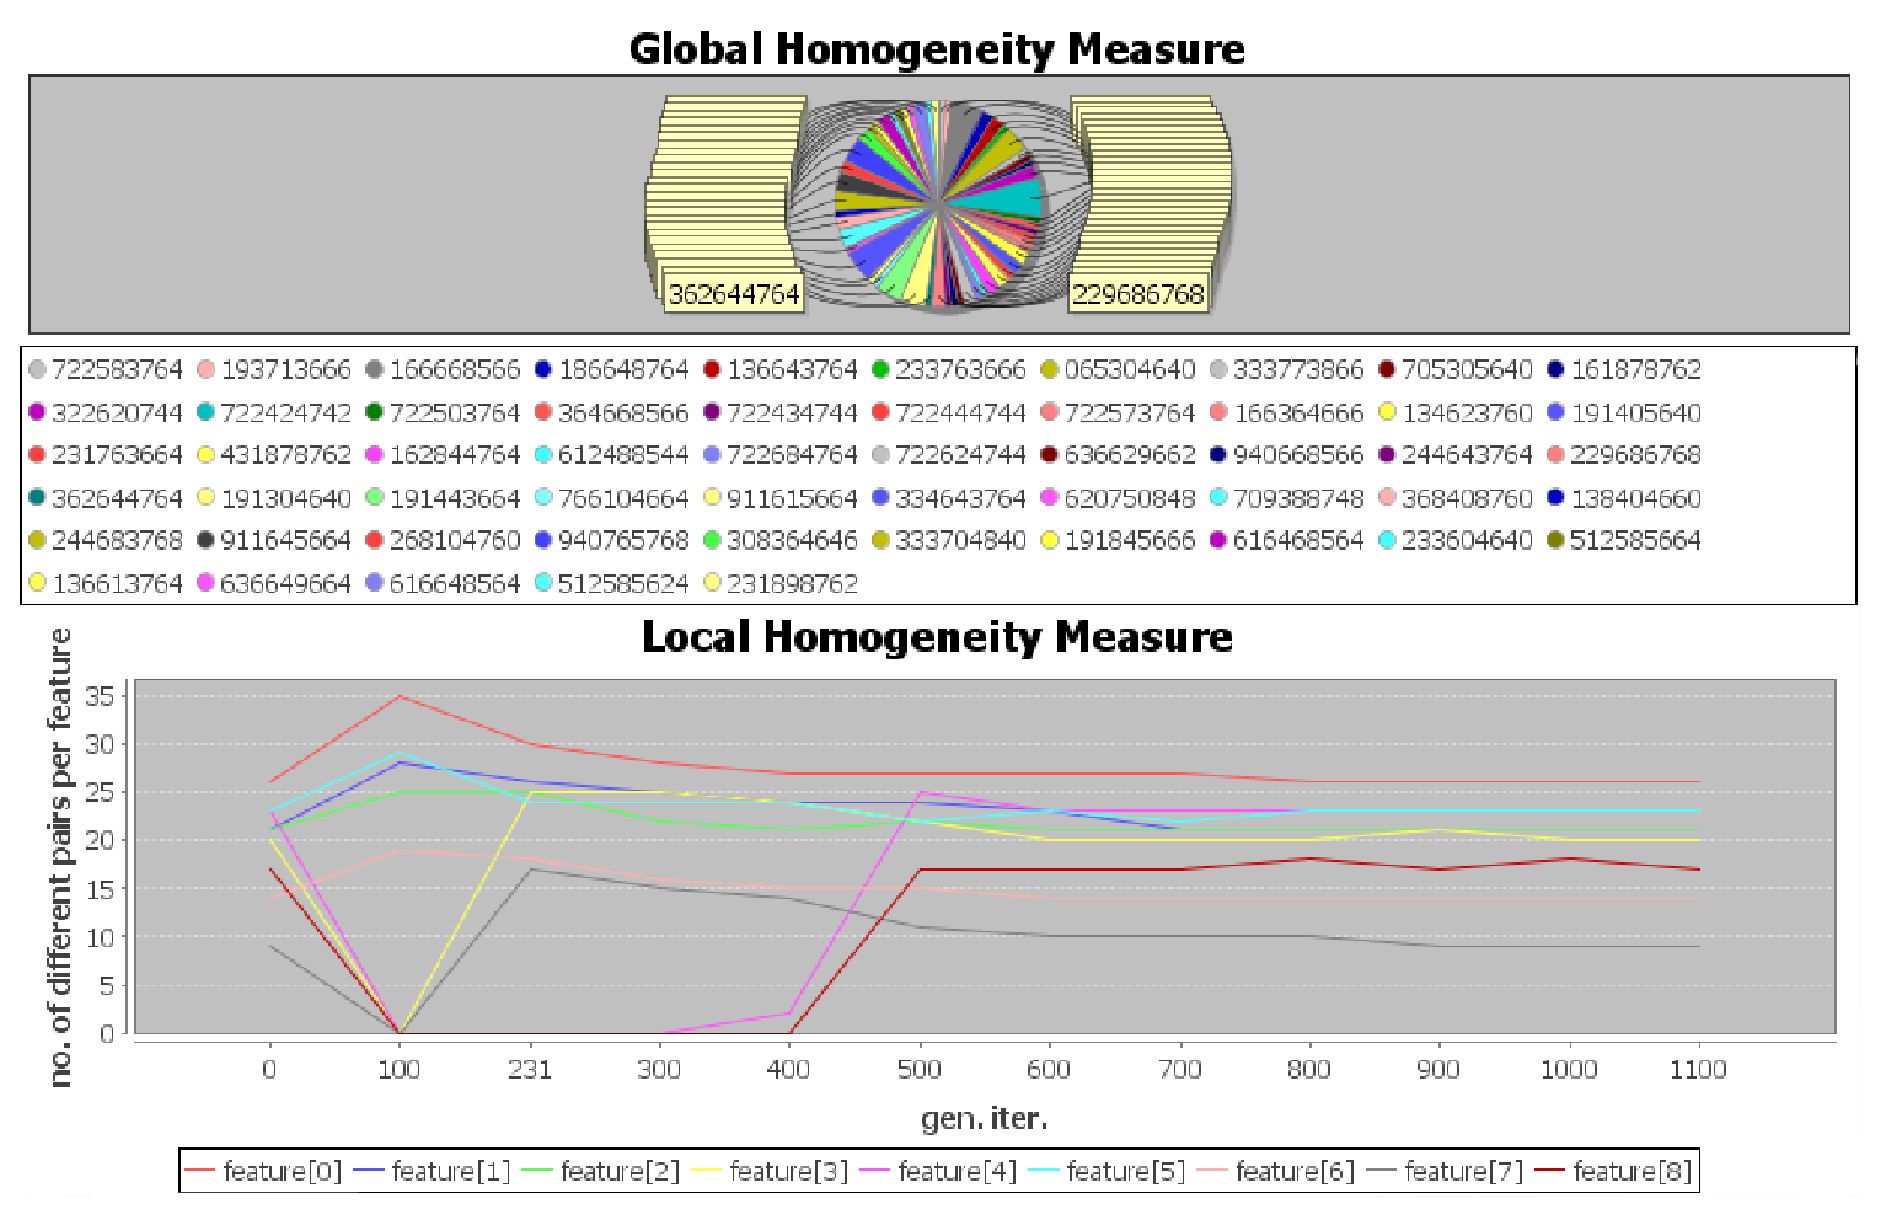
\includegraphics[width=\textwidth]{fig1}
		\caption{Complex simulation (with cultural attractiveness 0.9, 0.1)}
		\label{Fig 1}
\end{figure}

When removing the cultural attractiveness, and giving both internal and external features a probability of 1 to be changed, the number of generations until convergence slightly decreases.

If, however we set these probabilities to 0.5 each, convergence is reached later, and we could also notice how the number of values for each feature becomes uniformly distributed in the population (see figure 2).

\begin{figure}[htp]
		\centering
		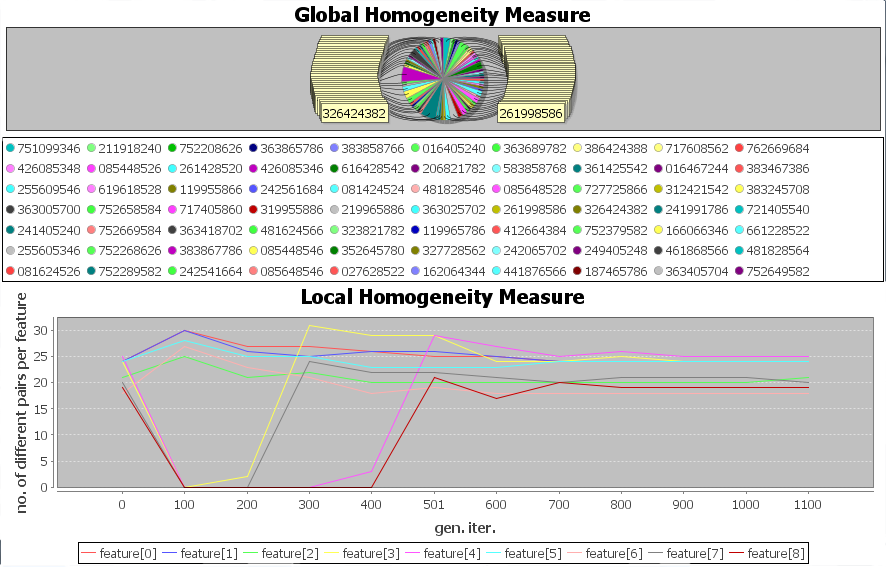
\includegraphics[width=\textwidth]{fig2}
		\caption{Complex simulation (without cultural attractivenes 0.5, 0.5)}
		\label{Fig 2}
\end{figure}


\section{Conclusions}

We ran three types of experiments, two of which were meant to offer a baseline for the third one. The baseline simulations generally followed the expected outcomes, as given in the related work we considered, though with some surprising turnovers. For instance, in the simple agent simulation, the size of the neighborhood and the imposed selection process actually leads to a destabilizing effect, i.e. the number of regions reaches a stable state, but the region boundaries change. Individuals end up having a single different feature, but due to the increased neighborhood size they keep exchanging the traits of that feature between them.
The surprise in the Balanced Agent experiment comes from the convergence speed. Given the fact that agents have to find a balance between their so called internal and external features, we would have expected the time the population takes to find stable solutions to be greater than what our simulations have shown.

The third and most interesting experiment showed what influence destabilizing factors, such as introducing new features or feature preference, have on measures like convergence speed and number of regions per feature. The influence on the total number of stable regions is yet to be analyzed.


\newpage
\pagebreak

\vskip 0.2in
\bibliographystyle{plain}
\bibliography{bibliography}

\end{document}

